\begin{activity} \label{A:11.6.10}  In this activity, we seek a
  parametrization of the sphere of radius $R$ centered at the origin, as
  shown on the left in Figure \ref{F:11.6.sphere}.  
  Notice that this sphere may be obtained by revolving a half-circle
  contained in the $xz$-plane about the $z$-axis, as shown on the right.

  \begin{figure}[ht]
    \begin{center}
      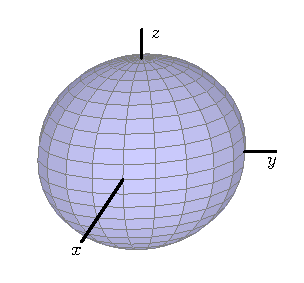
\includegraphics{figures/fig_11_6_sphere.eps}
      \hspace*{20pt}
      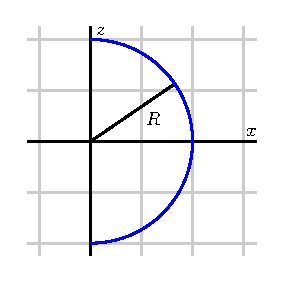
\includegraphics{figures/fig_11_6_sphere_half.eps}
    \end{center}
    \caption{A sphere obtained by revolving a half-circle.}
    \label{F:11.6.sphere}
  \end{figure}

  \ba
  \item Begin by writing a parametrization of this half-circle using
    the parameter $s$:
    $$
    x(s) = \ldots,\hspace*{20pt}
    z(s) = \ldots.
    $$
    Be sure to state the domain of the parameter $s$.
  \item By revolving the points on this half-circle about the
    $z$-axis, obtain a parametrization $\vr(s,t)$ of the points on the
    sphere of radius $R$.  Be sure to include the domain of both
    parameters $s$ and $t$. (Hint: What is the radius of the circle obtained when revolving a point on the half-circle around the $z$ axis?)

  \item Draw the surface defined by your parameterization with
    appropriate technology\footnote{e.g.,
    \url{http://web.monroecc.edu/manila/webfiles/calcNSF/JavaCode/CalcPlot3D.htm}
    or
    \url{http://www.flashandmath.com/mathlets/multicalc/paramrec/surf_graph_rectan.html}}.

    \ea



\end{activity}
\begin{smallhint}

\end{smallhint}
\begin{bighint}

\end{bighint}
\begin{activitySolution}
\ba
\item The parameterization of the half-circle is $x = R\cos(s)$, $y = 0$, $z=R\sin(s)$ for $-\frac{\pi}{2} \leq s \leq \frac{\pi}{2}$. 
\item A parameterization of the curve obtained by revolving the point $(R\cos(s), 0, R\sin(s))$ around the $z$-axis is $x=r\cos(t)$, $y=r\sin(t)$, $z=R\sin(s)$ for $0 \leq t \leq 2\pi$, where $r$ is the distance from the point to the $z$-axis. Note that this distance is just $R\cos(s)$, So a parameterization of the sphere of radius $R$ centered at the origin is 
\[\vr(s,t) = \langle R\cos(s)\cos(t), R\cos(s)\sin(t), R\sin(s) \rangle\]
for  $-\frac{\pi}{2} \leq s \leq \frac{\pi}{2}$ and $0 \leq t \leq 2\pi$. 
\ea

\end{activitySolution}
\aftera
